\hypertarget{interrupt_bare_8c-example}{}\section{interrupt\+\_\+bare.\+c}
Il file \hyperlink{interrupt__bare_8c}{interrupt\+\_\+bare.\+c} contiene un esempio d\textquotesingle{}uso del driver my\+G\+P\+IO bare-\/metal con interruzioni. L\textquotesingle{}esempio mostra come impostare il G\+IC affinché venga generata una interruzione, come debba essere servita, segnalando il completamento del servizio sia al G\+IC che al device my\+G\+P\+IO che ha generato l\textquotesingle{}interruzione.

\paragraph*{Configurazione hardware}

L\textquotesingle{}esempio fa riferimento ad una configurazione hardware in cui, oltre alla ip-\/core Zynq7000 processing sysyem, sono presenti tre diversi device my\+G\+P\+IO, uno connesso ai led (base address 0x43c00000), uno connesso ai button (base address 0x43c10000) ed uno connesso agli switch (base address 0x43c20000). Lo schema viene riportato di seguito\+:  
\begin{DoxyImageNoCaption}
  \mbox{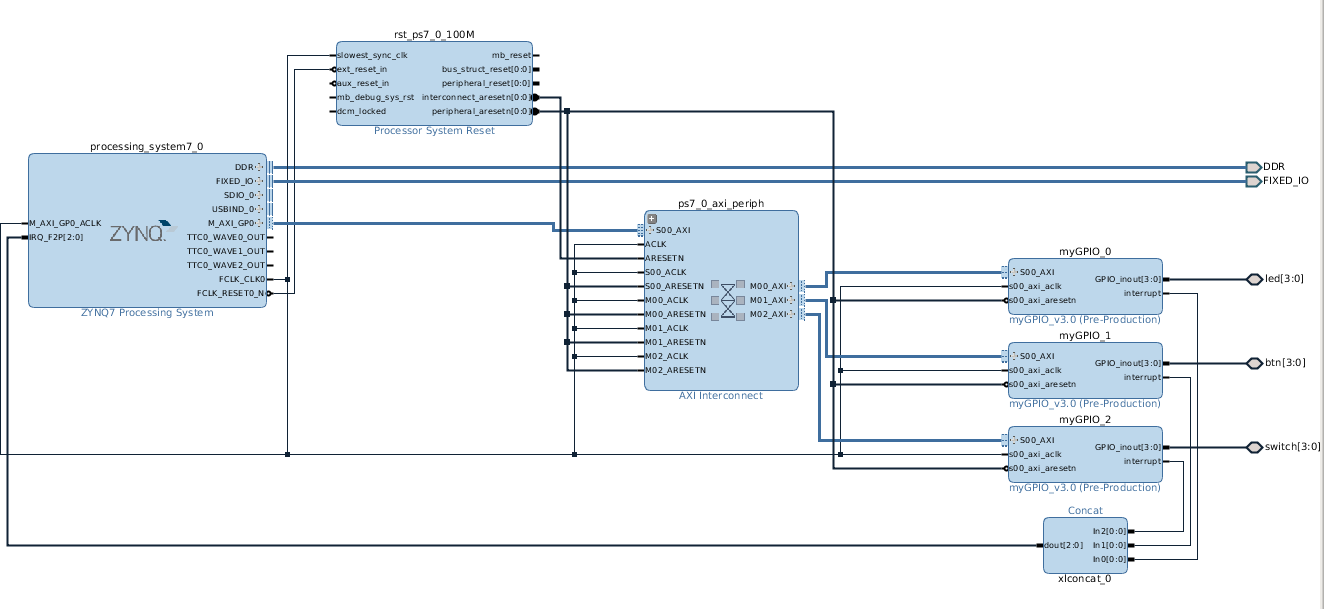
\includegraphics[width=\textwidth,height=\textheight/2,keepaspectratio=true]{interrupt_bare.png}}
\end{DoxyImageNoCaption}


\subparagraph*{I\+SR per la gestione di interrupt provenienti dal gpio connesso agli switch}


\begin{DoxyCode}
\textcolor{keywordtype}{void} \hyperlink{interrupt__bare_8c_ad05dc46b6c6da383d687c5116864b4ed}{swc\_isr}(\textcolor{keywordtype}{void}* data) \{
    \hyperlink{group__bare-metal_gaacca2871ac57a166e62bf431a2da7548}{myGPIO\_GlobalInterruptDisable}(&swc\_gpio);
    \hyperlink{group__bare-metal_ga402a0d20afc0cb7c25554b8b023f4253}{myGPIO\_mask} enabledInterrut = \hyperlink{group__bare-metal_ga80ef1cf3e9bd8bfd4d849a0f3b8e7b2c}{myGPIO\_EnabledPinInterrupt}(&swc\_gpio
      );
    \hyperlink{group__bare-metal_ga37d3df33ac50387d6f2e1fb5e2b13e49}{myGPIO\_PinInterruptDisable}(&swc\_gpio, enabledInterrut);

    \hyperlink{group__bare-metal_ga402a0d20afc0cb7c25554b8b023f4253}{myGPIO\_mask} pendingInterrupt = \hyperlink{group__bare-metal_ga6115bde39f860d4e76e7d8f421ce222c}{myGPIO\_PendingPinInterrupt}(&
      swc\_gpio);
    \hyperlink{group__bare-metal_gab6ad3dda867515825890c97dbf6f55db}{myGPIO\_PinInterruptAck}(&swc\_gpio, pendingInterrupt);

    \hyperlink{group__bare-metal_ga402a0d20afc0cb7c25554b8b023f4253}{myGPIO\_mask} value = \hyperlink{group__bare-metal_gac35776cd6652f7b932a132f3f6959a11}{myGPIO\_GetRead}(&swc\_gpio);
    \hyperlink{group__bare-metal_ga9d9ce9d2db7d77a588da4a3749f2f24d}{myGPIO\_SetValue}(&led\_gpio, \hyperlink{group__bare-metal_gga402a0d20afc0cb7c25554b8b023f4253a6db6fa7be955ae379f543d96122e23a9}{myGPIO\_pin0} | 
      \hyperlink{group__bare-metal_gga402a0d20afc0cb7c25554b8b023f4253a1de6bdcc01efca2c39f584f5a20293be}{myGPIO\_pin1} | \hyperlink{group__bare-metal_gga402a0d20afc0cb7c25554b8b023f4253a1fb3f52d920ac8ba17b74dd73c27d783}{myGPIO\_pin2} | \hyperlink{group__bare-metal_gga402a0d20afc0cb7c25554b8b023f4253a4514d64390392b626aa4dbfaac8dc1e5}{myGPIO\_pin3}, 
      \hyperlink{group__bare-metal_ggaf634fe4a0e1eab8da5000b72d6ad362ba98cde80dbda025bd1ae7231c76b55674}{myGPIO\_reset});
    \hyperlink{group__bare-metal_ga9d9ce9d2db7d77a588da4a3749f2f24d}{myGPIO\_SetValue}(&led\_gpio, value, \hyperlink{group__bare-metal_ggaf634fe4a0e1eab8da5000b72d6ad362ba10d296f3711d01189cc6c2d87f7c9149}{myGPIO\_set});

    \hyperlink{group__bare-metal_ga116e3a1077a317e9e42ded6dd4df64af}{myGPIO\_PinInterruptEnable}(&swc\_gpio, enabledInterrut);
    \hyperlink{group__bare-metal_gada93ef6a9818e634f0a233ce14582216}{myGPIO\_GlobalInterruptEnable}(&swc\_gpio);
\}
\end{DoxyCode}


La funzione di cui sopra non fa altro che disabilitare momentaneamente le interruzioni della periferica, leggere lo stato del registro “read”, resettare i led, per poi accendere solo quello corrispondente allo switch arrivo e riabilitare l\textquotesingle{}interrupt della periferica.

\subparagraph*{I\+SR per la gestione di interrupt provenienti dal gpio connesso ai button}


\begin{DoxyCode}
\textcolor{keywordtype}{void} \hyperlink{interrupt__bare_8c_aa4eac585cb67311e3e5fd374d6b09ad4}{btn\_isr}(\textcolor{keywordtype}{void}* data) \{
    \hyperlink{group__bare-metal_gaacca2871ac57a166e62bf431a2da7548}{myGPIO\_GlobalInterruptDisable}(&btn\_gpio);
    \hyperlink{group__bare-metal_ga402a0d20afc0cb7c25554b8b023f4253}{myGPIO\_mask} enabledInterrut = \hyperlink{group__bare-metal_ga80ef1cf3e9bd8bfd4d849a0f3b8e7b2c}{myGPIO\_EnabledPinInterrupt}(&btn\_gpio
      );
    \hyperlink{group__bare-metal_ga37d3df33ac50387d6f2e1fb5e2b13e49}{myGPIO\_PinInterruptDisable}(&btn\_gpio, enabledInterrut);

    \hyperlink{group__bare-metal_ga402a0d20afc0cb7c25554b8b023f4253}{myGPIO\_mask} pendingInterrupt = \hyperlink{group__bare-metal_ga6115bde39f860d4e76e7d8f421ce222c}{myGPIO\_PendingPinInterrupt}(&
      btn\_gpio);
    \hyperlink{group__bare-metal_gab6ad3dda867515825890c97dbf6f55db}{myGPIO\_PinInterruptAck}(&btn\_gpio, pendingInterrupt);

    \hyperlink{group__bare-metal_ga402a0d20afc0cb7c25554b8b023f4253}{myGPIO\_mask} value = \hyperlink{group__bare-metal_gac35776cd6652f7b932a132f3f6959a11}{myGPIO\_GetRead}(&btn\_gpio);
    \hyperlink{group__bare-metal_ga9d9ce9d2db7d77a588da4a3749f2f24d}{myGPIO\_SetValue}(&led\_gpio, \hyperlink{group__bare-metal_gga402a0d20afc0cb7c25554b8b023f4253a6db6fa7be955ae379f543d96122e23a9}{myGPIO\_pin0} | 
      \hyperlink{group__bare-metal_gga402a0d20afc0cb7c25554b8b023f4253a1de6bdcc01efca2c39f584f5a20293be}{myGPIO\_pin1} | \hyperlink{group__bare-metal_gga402a0d20afc0cb7c25554b8b023f4253a1fb3f52d920ac8ba17b74dd73c27d783}{myGPIO\_pin2} | \hyperlink{group__bare-metal_gga402a0d20afc0cb7c25554b8b023f4253a4514d64390392b626aa4dbfaac8dc1e5}{myGPIO\_pin3}, 
      \hyperlink{group__bare-metal_ggaf634fe4a0e1eab8da5000b72d6ad362ba98cde80dbda025bd1ae7231c76b55674}{myGPIO\_reset});
    \hyperlink{group__bare-metal_ga9d9ce9d2db7d77a588da4a3749f2f24d}{myGPIO\_SetValue}(&led\_gpio, value, \hyperlink{group__bare-metal_ggaf634fe4a0e1eab8da5000b72d6ad362ba10d296f3711d01189cc6c2d87f7c9149}{myGPIO\_set});

    \hyperlink{group__bare-metal_ga116e3a1077a317e9e42ded6dd4df64af}{myGPIO\_PinInterruptEnable}(&btn\_gpio, enabledInterrut);
    \hyperlink{group__bare-metal_gada93ef6a9818e634f0a233ce14582216}{myGPIO\_GlobalInterruptEnable}(&btn\_gpio);
\}
\end{DoxyCode}


La funzione di cui sopra non fa altro che disabilitare momentaneamente le interruzioni della periferica, leggere lo stato del registro “read”, resettare i led, per poi accendere solo quello corrispondente al button premuto e riabilitare l\textquotesingle{}interrupt della periferica.

\subparagraph*{Configurazione del G\+IC e registrazione degli interrupt handler}


\begin{DoxyCode}
\textcolor{keywordtype}{int} \hyperlink{interrupt__bare_8c_ad4c208e7b28dadf641bc3ec5b290d87d}{int\_config}(\textcolor{keywordtype}{void}) \{
    \textcolor{comment}{// inizializza il driver del GIC}
    Xil\_ExceptionInit();

    \textcolor{comment}{// ottiene i parametri di configurazione del GIC, lo configura ed inizializza}
    \textcolor{comment}{// sintassi : XScuGic\_LookupConfig(GIC\_id)}
    \textcolor{comment}{// sintassi : XScuGic\_CfgInitialize(GIC\_ptr, config, cpu\_address)}
    XScuGic\_Config *IntcConfig = XScuGic\_LookupConfig(\hyperlink{interrupt__bare_8c_a22782ed5aaa2e8d89334d159d14753b5}{gic\_id});
    \textcolor{keywordflow}{if} (IntcConfig == NULL)
        \textcolor{keywordflow}{return} -1;
    \textcolor{keywordflow}{if} (XScuGic\_CfgInitialize(&\hyperlink{interrupt__bare_8c_a0ad1175dbe99ac3f36c814258ec4f8c6}{GIC}, IntcConfig, IntcConfig->CpuBaseAddress) != XST\_SUCCESS)
        \textcolor{keywordflow}{return} -1;

    \textcolor{comment}{// registra l'interrupt handler del GIC alla logica di gestione del processing-system}
    \textcolor{comment}{// sintassi : Xil\_ExceptionRegisterHandler(XIL\_EXCEPTION\_ID\_INT, handler, gic\_ptr)}
    Xil\_ExceptionRegisterHandler(XIL\_EXCEPTION\_ID\_INT,(Xil\_ExceptionHandler)XScuGic\_InterruptHandler, &
      \hyperlink{interrupt__bare_8c_a0ad1175dbe99ac3f36c814258ec4f8c6}{GIC});

    \textcolor{comment}{// registrazione degli handler}
    \textcolor{comment}{// le righe seguenti stabiliscono quale sia l'handler da chiamare e quali dati bisogna passargli}
    \textcolor{comment}{// qualora si manifesti una interruzione su una line di irq.}
    \textcolor{comment}{// sintassi : XScuGic\_Connect(GIC, irq\_line, handler, data)}
    \textcolor{keywordflow}{if} (XScuGic\_Connect(&\hyperlink{interrupt__bare_8c_a0ad1175dbe99ac3f36c814258ec4f8c6}{GIC}, \hyperlink{interrupt__bare_8c_ab5602e3672ec6d03f39d2229dbcb9f74}{btn\_irq\_line}, (Xil\_InterruptHandler)btn\_isr, (\textcolor{keywordtype}{void}*)NULL) != 
      XST\_SUCCESS)
        \textcolor{keywordflow}{return} -1;
    \textcolor{keywordflow}{if} (XScuGic\_Connect(&\hyperlink{interrupt__bare_8c_a0ad1175dbe99ac3f36c814258ec4f8c6}{GIC}, \hyperlink{interrupt__bare_8c_a48d05dc71b54a160af13c8e31e9000b1}{swc\_irq\_line}, (Xil\_InterruptHandler)swc\_isr, (\textcolor{keywordtype}{void}*)NULL) != 
      XST\_SUCCESS)
            \textcolor{keywordflow}{return} -1;

    \textcolor{comment}{// abilitazione degli interrupt sulle linee connesse alle periferiche}
    \textcolor{comment}{// sintassi: XScuGic\_Enable(GIC,irq\_line);}
    XScuGic\_Enable(&\hyperlink{interrupt__bare_8c_a0ad1175dbe99ac3f36c814258ec4f8c6}{GIC}, \hyperlink{interrupt__bare_8c_ab5602e3672ec6d03f39d2229dbcb9f74}{btn\_irq\_line});
    XScuGic\_Enable(&\hyperlink{interrupt__bare_8c_a0ad1175dbe99ac3f36c814258ec4f8c6}{GIC}, \hyperlink{interrupt__bare_8c_a48d05dc71b54a160af13c8e31e9000b1}{swc\_irq\_line});

    \textcolor{comment}{// abilitazione degli interrupt delle periferiche}
    \hyperlink{group__bare-metal_gada93ef6a9818e634f0a233ce14582216}{myGPIO\_GlobalInterruptEnable}(&btn\_gpio);
    \hyperlink{group__bare-metal_ga116e3a1077a317e9e42ded6dd4df64af}{myGPIO\_PinInterruptEnable}(&btn\_gpio, \hyperlink{group__bare-metal_gga402a0d20afc0cb7c25554b8b023f4253a6db6fa7be955ae379f543d96122e23a9}{myGPIO\_pin0} | 
      \hyperlink{group__bare-metal_gga402a0d20afc0cb7c25554b8b023f4253a1de6bdcc01efca2c39f584f5a20293be}{myGPIO\_pin1} | \hyperlink{group__bare-metal_gga402a0d20afc0cb7c25554b8b023f4253a1fb3f52d920ac8ba17b74dd73c27d783}{myGPIO\_pin2} | \hyperlink{group__bare-metal_gga402a0d20afc0cb7c25554b8b023f4253a4514d64390392b626aa4dbfaac8dc1e5}{myGPIO\_pin3});
    \hyperlink{group__bare-metal_gada93ef6a9818e634f0a233ce14582216}{myGPIO\_GlobalInterruptEnable}(&swc\_gpio);
    \hyperlink{group__bare-metal_ga116e3a1077a317e9e42ded6dd4df64af}{myGPIO\_PinInterruptEnable}(&swc\_gpio, \hyperlink{group__bare-metal_gga402a0d20afc0cb7c25554b8b023f4253a6db6fa7be955ae379f543d96122e23a9}{myGPIO\_pin0} | 
      \hyperlink{group__bare-metal_gga402a0d20afc0cb7c25554b8b023f4253a1de6bdcc01efca2c39f584f5a20293be}{myGPIO\_pin1} | \hyperlink{group__bare-metal_gga402a0d20afc0cb7c25554b8b023f4253a1fb3f52d920ac8ba17b74dd73c27d783}{myGPIO\_pin2} | \hyperlink{group__bare-metal_gga402a0d20afc0cb7c25554b8b023f4253a4514d64390392b626aa4dbfaac8dc1e5}{myGPIO\_pin3});

    \textcolor{comment}{// abilitazione degli interrupt del processing-system}
    Xil\_ExceptionEnable();
    \textcolor{keywordflow}{return} 0;
\}
\end{DoxyCode}
 La funzione di configurazione delle interrupt e del G\+IC fa uso di alcune funzioni di libreria definite nell\textquotesingle{}header file \char`\"{}xscugic.\+h\char`\"{}, il quale implementa il driver della periferica G\+IC, e di alcune macro definite nel file \char`\"{}xparameters.\+h\char`\"{}. Solo per comodità le macro definite in xparameters.\+h sono state ridefinite come segue. 
\begin{DoxyCode}
\textcolor{preprocessor}{#define led\_base\_addr XPAR\_MYGPIO\_0\_S00\_AXI\_BASEADDR}
\textcolor{preprocessor}{#define btn\_base\_addr XPAR\_MYGPIO\_1\_S00\_AXI\_BASEADDR}
\textcolor{preprocessor}{#define swc\_base\_addr XPAR\_MYGPIO\_2\_S00\_AXI\_BASEADDR}
\textcolor{preprocessor}{#define led\_irq\_line XPAR\_FABRIC\_MYGPIO\_0\_INTERRUPT\_INTR}
\textcolor{preprocessor}{#define btn\_irq\_line XPAR\_FABRIC\_MYGPIO\_1\_INTERRUPT\_INTR}
\textcolor{preprocessor}{#define swc\_irq\_line XPAR\_FABRIC\_MYGPIO\_2\_INTERRUPT\_INTR}
\textcolor{preprocessor}{#define gic\_id      XPAR\_SCUGIC\_0\_DEVICE\_ID}
\end{DoxyCode}
 Le funzioni di libreria usate sono riportate di seguito, assieme ad una breve descrizione tratta dalla documentazione interna.
\begin{DoxyItemize}
\item Xil\+\_\+\+Exception\+Init()\+: inizializza gli exception-\/handlers di tutti i processori. Per A\+RM Cortex A53, R5 ed A9 gli exception-\/handlers sono sono inizializzati staticamente, per cui questa funzione non fa niente. Viene mantenutaper prevenire errori in fase di compilazione e per garantire backward-\/compatibility.
\item X\+Scu\+Gic\+\_\+\+Lookup\+Config()\+: looksup della configurazione di un device, basandosi sull\textquotesingle{}identificativo univoco dello stesso, dalla tabella contenente le configurazioni di tutti i device. Prende in ingresso un parametro Device\+Id e restituisce un puntatore a X\+Scu\+Gic, contenente la configurazione, o N\+U\+LL se il device non viene trovato.
\item X\+Scu\+Gic\+\_\+\+Cfg\+Initialize()\+: inizializza e configura un interrupt-\/controller instance/driver. La procedura di inizializzazione prevede\+:
\begin{DoxyItemize}
\item l\textquotesingle{}inizializzazione dei campi di una struttura X\+Scu\+Gic;
\item la configurazione della Initial vector-\/table, con funzioni stub;
\item disabilitazione di tutte le sorgenti di interruzione
\end{DoxyItemize}Parametri\+:
\begin{DoxyItemize}
\item Instance\+Ptr\+: puntatore a struttura X\+Scu\+Gic;
\item Config\+Ptr\+: puntatore alla configurazione del device, restituito dalla funzione X\+Scu\+Gic\+\_\+\+Lookup\+Config();
\item Effective\+Addr\+: indirizzo base del device; Restituisce X\+S\+T\+\_\+\+S\+U\+C\+C\+E\+SS se l\textquotesingle{}inizializzazione viene completata con successo.
\end{DoxyItemize}
\item Xil\+\_\+\+Exception\+Register\+Handler()\+: crea una connessione tra l\textquotesingle{}identificativo di una sorgente di eccezioni e l\textquotesingle{}handler associato, in modo che l\textquotesingle{}handler venga eseguito qualora si manifestasse una eccezione. Prende i seguenti parametri\+:
\begin{DoxyItemize}
\item exception\+\_\+id\+: ID della sorgente di eccezioni;
\item Handler\+: puntatore alla funzione di servizio;
\item Data\+: puntatore ai dati da passare all\textquotesingle{}handler;
\end{DoxyItemize}
\item X\+Scu\+Gic\+\_\+\+Connect()\+: crea una connessione tra l\textquotesingle{}identificativo di una sorgente di interruzioni e l\textquotesingle{}handler associato, in modo che l\textquotesingle{}handler venga eseguito qualora si manifestasse una interruzione. Prende i seguenti parametri\+:
\begin{DoxyItemize}
\item Instance\+Ptr\+: puntatore ad una istanza X\+Scu\+Gic;
\item Int\+\_\+\+Id\+: ID della sorgente di interruzioni;
\item Handler\+: puntatore alla funzione di servizio;
\item Call\+Back\+Ref\+: puntatore ai dati da passare alla isr;
\end{DoxyItemize}Restituisce X\+S\+T\+\_\+\+S\+U\+C\+C\+E\+SS se l\textquotesingle{}handler è stato connesso correttamente.
\item X\+Scu\+Gic\+\_\+\+Enable()\+: abilita la sorgente di interruzioni Int\+\_\+\+Id. Se ci sono pending interrupt per tale linea, scateneranno una interruzione dopo la chiamata a questa funzione. Parametri\+:
\begin{DoxyItemize}
\item Instance\+Ptr\+: puntatore ad una istanza X\+Scu\+Gic;
\item Int\+\_\+\+Id\+: ID della sorgente di interruzioni;
\end{DoxyItemize}
\item Xil\+\_\+\+Exception\+Enable()\+: abilita le interruzioni.
\end{DoxyItemize}


\begin{DoxyCodeInclude}

\textcolor{preprocessor}{#include "xparameters.h"}
\textcolor{preprocessor}{#include "xscugic.h"}
\textcolor{preprocessor}{#include "\hyperlink{my_g_p_i_o_8h}{myGPIO.h}"}

\hyperlink{structmy_g_p_i_o__t}{myGPIO\_t} \hyperlink{interrupt__bare_8c_ac523aaaf082570c199faf2a98e03c219}{led\_gpio};
\hyperlink{structmy_g_p_i_o__t}{myGPIO\_t} \hyperlink{interrupt__bare_8c_ac77d5df697b8a0d64704dee5f1433832}{btn\_gpio};
\hyperlink{structmy_g_p_i_o__t}{myGPIO\_t} \hyperlink{interrupt__bare_8c_ac2f1233c00752afeb2ecfd305c5fe36a}{swc\_gpio};
XScuGic \hyperlink{interrupt__bare_8c_a0ad1175dbe99ac3f36c814258ec4f8c6}{GIC};

\textcolor{preprocessor}{#define led\_base\_addr XPAR\_MYGPIO\_0\_S00\_AXI\_BASEADDR}
\textcolor{preprocessor}{#define btn\_base\_addr XPAR\_MYGPIO\_1\_S00\_AXI\_BASEADDR}
\textcolor{preprocessor}{#define swc\_base\_addr XPAR\_MYGPIO\_2\_S00\_AXI\_BASEADDR}

\textcolor{preprocessor}{#define led\_irq\_line XPAR\_FABRIC\_MYGPIO\_0\_INTERRUPT\_INTR}
\textcolor{preprocessor}{#define btn\_irq\_line XPAR\_FABRIC\_MYGPIO\_1\_INTERRUPT\_INTR}
\textcolor{preprocessor}{#define swc\_irq\_line XPAR\_FABRIC\_MYGPIO\_2\_INTERRUPT\_INTR}

\textcolor{preprocessor}{#define gic\_id      XPAR\_SCUGIC\_0\_DEVICE\_ID}

\textcolor{comment}{// funzione di inizializzazione dei device gpio}
\textcolor{keywordtype}{void} \hyperlink{interrupt__bare_8c_afdbe206b3c49f019757ab09b3cf52b9c}{gpio\_init}(\textcolor{keywordtype}{void});

\textcolor{comment}{// isr per button e switch}
\textcolor{comment}{// devono necessariamente avere questa firma: restituire void e possedere un solo parametro puntatore}
\textcolor{comment}{// a void. In questo caso non viene utilizzato (tutte le variabili sono globali), ma tale puntatore}
\textcolor{comment}{// può essere usato per scambiare dati di ingresso/uscita alle isr}
\textcolor{keywordtype}{void} \hyperlink{interrupt__bare_8c_aa4eac585cb67311e3e5fd374d6b09ad4}{btn\_isr}(\textcolor{keywordtype}{void}*); \textcolor{comment}{// isr per i button}
\textcolor{keywordtype}{void} \hyperlink{interrupt__bare_8c_ad05dc46b6c6da383d687c5116864b4ed}{swc\_isr}(\textcolor{keywordtype}{void}*); \textcolor{comment}{// isr per gli switch}

\textcolor{comment}{// funzione di configurazione del device gic e delle interruzioni}
\textcolor{keywordtype}{int} \hyperlink{interrupt__bare_8c_ad4c208e7b28dadf641bc3ec5b290d87d}{int\_config}(\textcolor{keywordtype}{void});

\textcolor{keywordtype}{int} \hyperlink{interrupt__bare_8c_ae66f6b31b5ad750f1fe042a706a4e3d4}{main}() \{
    \hyperlink{interrupt__bare_8c_afdbe206b3c49f019757ab09b3cf52b9c}{gpio\_init}();
    \hyperlink{interrupt__bare_8c_ad4c208e7b28dadf641bc3ec5b290d87d}{int\_config}();
    \textcolor{keywordflow}{for} (;;);
    \textcolor{keywordflow}{return} 0;
\}

\textcolor{keywordtype}{void} \hyperlink{interrupt__bare_8c_afdbe206b3c49f019757ab09b3cf52b9c}{gpio\_init}(\textcolor{keywordtype}{void}) \{
    uint8\_t i;

    \hyperlink{group__bare-metal_ga588201358d1633c53535b288c9198531}{myGPIO\_Init}(&led\_gpio, \hyperlink{interrupt__bare_8c_a145e4211eed7013a18d03ed032f0f229}{led\_base\_addr});
    \hyperlink{group__bare-metal_ga588201358d1633c53535b288c9198531}{myGPIO\_Init}(&btn\_gpio, \hyperlink{interrupt__bare_8c_aedc39629300adb6d9f8b1359eb2f7024}{btn\_base\_addr});
    \hyperlink{group__bare-metal_ga588201358d1633c53535b288c9198531}{myGPIO\_Init}(&swc\_gpio, \hyperlink{interrupt__bare_8c_a0f79b2ec9c50221371b1a5c027654774}{swc\_base\_addr});
    \textcolor{keywordflow}{for} (i=0; i<4; i++) \{
        \hyperlink{group__bare-metal_ga43e82eb0febd452635a438fbd9cb853b}{myGPIO\_SetMode}(&led\_gpio, \hyperlink{group__bare-metal_gabbe2491a3b71c292521025b7b382b971}{myGPIO\_pin}(i), 
      \hyperlink{group__bare-metal_gga76b849f0e0c05e7f9161bdb33396f2b1a2d66976280eb7595a42c631683bdfad6}{myGPIO\_write});
        \hyperlink{group__bare-metal_ga9d9ce9d2db7d77a588da4a3749f2f24d}{myGPIO\_SetValue}(&led\_gpio, \hyperlink{group__bare-metal_gabbe2491a3b71c292521025b7b382b971}{myGPIO\_pin}(i), 
      \hyperlink{group__bare-metal_ggaf634fe4a0e1eab8da5000b72d6ad362ba98cde80dbda025bd1ae7231c76b55674}{myGPIO\_reset});
        \hyperlink{group__bare-metal_ga43e82eb0febd452635a438fbd9cb853b}{myGPIO\_SetMode}(&btn\_gpio, \hyperlink{group__bare-metal_gabbe2491a3b71c292521025b7b382b971}{myGPIO\_pin}(i), 
      \hyperlink{group__bare-metal_gga76b849f0e0c05e7f9161bdb33396f2b1a1e6dc78e7641e878cadc842d39605d5d}{myGPIO\_read});
        \hyperlink{group__bare-metal_ga9d9ce9d2db7d77a588da4a3749f2f24d}{myGPIO\_SetValue}(&btn\_gpio, \hyperlink{group__bare-metal_gabbe2491a3b71c292521025b7b382b971}{myGPIO\_pin}(i), 
      \hyperlink{group__bare-metal_ggaf634fe4a0e1eab8da5000b72d6ad362ba98cde80dbda025bd1ae7231c76b55674}{myGPIO\_reset});
        \hyperlink{group__bare-metal_ga43e82eb0febd452635a438fbd9cb853b}{myGPIO\_SetMode}(&swc\_gpio, \hyperlink{group__bare-metal_gabbe2491a3b71c292521025b7b382b971}{myGPIO\_pin}(i), 
      \hyperlink{group__bare-metal_gga76b849f0e0c05e7f9161bdb33396f2b1a1e6dc78e7641e878cadc842d39605d5d}{myGPIO\_read});
        \hyperlink{group__bare-metal_ga9d9ce9d2db7d77a588da4a3749f2f24d}{myGPIO\_SetValue}(&swc\_gpio, \hyperlink{group__bare-metal_gabbe2491a3b71c292521025b7b382b971}{myGPIO\_pin}(i), 
      \hyperlink{group__bare-metal_ggaf634fe4a0e1eab8da5000b72d6ad362ba98cde80dbda025bd1ae7231c76b55674}{myGPIO\_reset});
    \}
\}

\textcolor{keywordtype}{void} \hyperlink{interrupt__bare_8c_aa4eac585cb67311e3e5fd374d6b09ad4}{btn\_isr}(\textcolor{keywordtype}{void}* data) \{
    \hyperlink{group__bare-metal_gaacca2871ac57a166e62bf431a2da7548}{myGPIO\_GlobalInterruptDisable}(&btn\_gpio);
    \hyperlink{group__bare-metal_ga402a0d20afc0cb7c25554b8b023f4253}{myGPIO\_mask} enabledInterrut = \hyperlink{group__bare-metal_ga80ef1cf3e9bd8bfd4d849a0f3b8e7b2c}{myGPIO\_EnabledPinInterrupt}(&btn\_gpio
      );
    \hyperlink{group__bare-metal_ga37d3df33ac50387d6f2e1fb5e2b13e49}{myGPIO\_PinInterruptDisable}(&btn\_gpio, enabledInterrut);

    \hyperlink{group__bare-metal_ga402a0d20afc0cb7c25554b8b023f4253}{myGPIO\_mask} pendingInterrupt = \hyperlink{group__bare-metal_ga6115bde39f860d4e76e7d8f421ce222c}{myGPIO\_PendingPinInterrupt}(&
      btn\_gpio);
    \hyperlink{group__bare-metal_gab6ad3dda867515825890c97dbf6f55db}{myGPIO\_PinInterruptAck}(&btn\_gpio, pendingInterrupt);

    \hyperlink{group__bare-metal_ga402a0d20afc0cb7c25554b8b023f4253}{myGPIO\_mask} value = \hyperlink{group__bare-metal_gac35776cd6652f7b932a132f3f6959a11}{myGPIO\_GetRead}(&btn\_gpio);
    \hyperlink{group__bare-metal_ga9d9ce9d2db7d77a588da4a3749f2f24d}{myGPIO\_SetValue}(&led\_gpio, \hyperlink{group__bare-metal_gga402a0d20afc0cb7c25554b8b023f4253a6db6fa7be955ae379f543d96122e23a9}{myGPIO\_pin0} | 
      \hyperlink{group__bare-metal_gga402a0d20afc0cb7c25554b8b023f4253a1de6bdcc01efca2c39f584f5a20293be}{myGPIO\_pin1} | \hyperlink{group__bare-metal_gga402a0d20afc0cb7c25554b8b023f4253a1fb3f52d920ac8ba17b74dd73c27d783}{myGPIO\_pin2} | \hyperlink{group__bare-metal_gga402a0d20afc0cb7c25554b8b023f4253a4514d64390392b626aa4dbfaac8dc1e5}{myGPIO\_pin3}, 
      \hyperlink{group__bare-metal_ggaf634fe4a0e1eab8da5000b72d6ad362ba98cde80dbda025bd1ae7231c76b55674}{myGPIO\_reset});
    \hyperlink{group__bare-metal_ga9d9ce9d2db7d77a588da4a3749f2f24d}{myGPIO\_SetValue}(&led\_gpio, value, \hyperlink{group__bare-metal_ggaf634fe4a0e1eab8da5000b72d6ad362ba10d296f3711d01189cc6c2d87f7c9149}{myGPIO\_set});

    \hyperlink{group__bare-metal_ga116e3a1077a317e9e42ded6dd4df64af}{myGPIO\_PinInterruptEnable}(&btn\_gpio, enabledInterrut);
    \hyperlink{group__bare-metal_gada93ef6a9818e634f0a233ce14582216}{myGPIO\_GlobalInterruptEnable}(&btn\_gpio);
\}

\textcolor{keywordtype}{void} \hyperlink{interrupt__bare_8c_ad05dc46b6c6da383d687c5116864b4ed}{swc\_isr}(\textcolor{keywordtype}{void}* data) \{
    \hyperlink{group__bare-metal_gaacca2871ac57a166e62bf431a2da7548}{myGPIO\_GlobalInterruptDisable}(&swc\_gpio);
    \hyperlink{group__bare-metal_ga402a0d20afc0cb7c25554b8b023f4253}{myGPIO\_mask} enabledInterrut = \hyperlink{group__bare-metal_ga80ef1cf3e9bd8bfd4d849a0f3b8e7b2c}{myGPIO\_EnabledPinInterrupt}(&swc\_gpio
      );
    \hyperlink{group__bare-metal_ga37d3df33ac50387d6f2e1fb5e2b13e49}{myGPIO\_PinInterruptDisable}(&swc\_gpio, enabledInterrut);

    \hyperlink{group__bare-metal_ga402a0d20afc0cb7c25554b8b023f4253}{myGPIO\_mask} pendingInterrupt = \hyperlink{group__bare-metal_ga6115bde39f860d4e76e7d8f421ce222c}{myGPIO\_PendingPinInterrupt}(&
      swc\_gpio);
    \hyperlink{group__bare-metal_gab6ad3dda867515825890c97dbf6f55db}{myGPIO\_PinInterruptAck}(&swc\_gpio, pendingInterrupt);

    \hyperlink{group__bare-metal_ga402a0d20afc0cb7c25554b8b023f4253}{myGPIO\_mask} value = \hyperlink{group__bare-metal_gac35776cd6652f7b932a132f3f6959a11}{myGPIO\_GetRead}(&swc\_gpio);
    \hyperlink{group__bare-metal_ga9d9ce9d2db7d77a588da4a3749f2f24d}{myGPIO\_SetValue}(&led\_gpio, \hyperlink{group__bare-metal_gga402a0d20afc0cb7c25554b8b023f4253a6db6fa7be955ae379f543d96122e23a9}{myGPIO\_pin0} | 
      \hyperlink{group__bare-metal_gga402a0d20afc0cb7c25554b8b023f4253a1de6bdcc01efca2c39f584f5a20293be}{myGPIO\_pin1} | \hyperlink{group__bare-metal_gga402a0d20afc0cb7c25554b8b023f4253a1fb3f52d920ac8ba17b74dd73c27d783}{myGPIO\_pin2} | \hyperlink{group__bare-metal_gga402a0d20afc0cb7c25554b8b023f4253a4514d64390392b626aa4dbfaac8dc1e5}{myGPIO\_pin3}, 
      \hyperlink{group__bare-metal_ggaf634fe4a0e1eab8da5000b72d6ad362ba98cde80dbda025bd1ae7231c76b55674}{myGPIO\_reset});
    \hyperlink{group__bare-metal_ga9d9ce9d2db7d77a588da4a3749f2f24d}{myGPIO\_SetValue}(&led\_gpio, value, \hyperlink{group__bare-metal_ggaf634fe4a0e1eab8da5000b72d6ad362ba10d296f3711d01189cc6c2d87f7c9149}{myGPIO\_set});

    \hyperlink{group__bare-metal_ga116e3a1077a317e9e42ded6dd4df64af}{myGPIO\_PinInterruptEnable}(&swc\_gpio, enabledInterrut);
    \hyperlink{group__bare-metal_gada93ef6a9818e634f0a233ce14582216}{myGPIO\_GlobalInterruptEnable}(&swc\_gpio);
\}

\textcolor{keywordtype}{int} \hyperlink{interrupt__bare_8c_ad4c208e7b28dadf641bc3ec5b290d87d}{int\_config}(\textcolor{keywordtype}{void}) \{
    \textcolor{comment}{// inizializza il driver del GIC}
    Xil\_ExceptionInit();

    \textcolor{comment}{// ottiene i parametri di configurazione del GIC, lo configura ed inizializza}
    \textcolor{comment}{// sintassi : XScuGic\_LookupConfig(GIC\_id)}
    \textcolor{comment}{// sintassi : XScuGic\_CfgInitialize(GIC\_ptr, config, cpu\_address)}
    XScuGic\_Config *IntcConfig = XScuGic\_LookupConfig(\hyperlink{interrupt__bare_8c_a22782ed5aaa2e8d89334d159d14753b5}{gic\_id});
    \textcolor{keywordflow}{if} (IntcConfig == NULL)
        \textcolor{keywordflow}{return} -1;
    \textcolor{keywordflow}{if} (XScuGic\_CfgInitialize(&GIC, IntcConfig, IntcConfig->CpuBaseAddress) != XST\_SUCCESS)
        \textcolor{keywordflow}{return} -1;

    \textcolor{comment}{// registra l'interrupt handler del GIC alla logica di gestione del processing-system}
    \textcolor{comment}{// sintassi : Xil\_ExceptionRegisterHandler(XIL\_EXCEPTION\_ID\_INT, handler, gic\_ptr)}
    Xil\_ExceptionRegisterHandler(XIL\_EXCEPTION\_ID\_INT,(Xil\_ExceptionHandler)XScuGic\_InterruptHandler, &GIC)
      ;

    \textcolor{comment}{// registrazione degli handler}
    \textcolor{comment}{// le righe seguenti stabiliscono quale sia l'handler da chiamare e quali dati bisogna passargli}
    \textcolor{comment}{// qualora si manifesti una interruzione su una line di irq.}
    \textcolor{comment}{// sintassi : XScuGic\_Connect(GIC, irq\_line, handler, data)}
    \textcolor{keywordflow}{if} (XScuGic\_Connect(&GIC, \hyperlink{interrupt__bare_8c_ab5602e3672ec6d03f39d2229dbcb9f74}{btn\_irq\_line}, (Xil\_InterruptHandler)btn\_isr, (\textcolor{keywordtype}{void}*)NULL) != 
      XST\_SUCCESS)
        \textcolor{keywordflow}{return} -1;
    \textcolor{keywordflow}{if} (XScuGic\_Connect(&GIC, \hyperlink{interrupt__bare_8c_a48d05dc71b54a160af13c8e31e9000b1}{swc\_irq\_line}, (Xil\_InterruptHandler)swc\_isr, (\textcolor{keywordtype}{void}*)NULL) != 
      XST\_SUCCESS)
            \textcolor{keywordflow}{return} -1;

    \textcolor{comment}{// abilitazione degli interrupt sulle linee connesse alle periferiche}
    \textcolor{comment}{// sintassi: XScuGic\_Enable(GIC,irq\_line);}
    XScuGic\_Enable(&GIC, \hyperlink{interrupt__bare_8c_ab5602e3672ec6d03f39d2229dbcb9f74}{btn\_irq\_line});
    XScuGic\_Enable(&GIC, \hyperlink{interrupt__bare_8c_a48d05dc71b54a160af13c8e31e9000b1}{swc\_irq\_line});

    \textcolor{comment}{// abilitazione degli interrupt delle periferiche}
    \hyperlink{group__bare-metal_gada93ef6a9818e634f0a233ce14582216}{myGPIO\_GlobalInterruptEnable}(&btn\_gpio);
    \hyperlink{group__bare-metal_ga116e3a1077a317e9e42ded6dd4df64af}{myGPIO\_PinInterruptEnable}(&btn\_gpio, \hyperlink{group__bare-metal_gga402a0d20afc0cb7c25554b8b023f4253a6db6fa7be955ae379f543d96122e23a9}{myGPIO\_pin0} | 
      \hyperlink{group__bare-metal_gga402a0d20afc0cb7c25554b8b023f4253a1de6bdcc01efca2c39f584f5a20293be}{myGPIO\_pin1} | \hyperlink{group__bare-metal_gga402a0d20afc0cb7c25554b8b023f4253a1fb3f52d920ac8ba17b74dd73c27d783}{myGPIO\_pin2} | \hyperlink{group__bare-metal_gga402a0d20afc0cb7c25554b8b023f4253a4514d64390392b626aa4dbfaac8dc1e5}{myGPIO\_pin3});
    \hyperlink{group__bare-metal_gada93ef6a9818e634f0a233ce14582216}{myGPIO\_GlobalInterruptEnable}(&swc\_gpio);
    \hyperlink{group__bare-metal_ga116e3a1077a317e9e42ded6dd4df64af}{myGPIO\_PinInterruptEnable}(&swc\_gpio, \hyperlink{group__bare-metal_gga402a0d20afc0cb7c25554b8b023f4253a6db6fa7be955ae379f543d96122e23a9}{myGPIO\_pin0} | 
      \hyperlink{group__bare-metal_gga402a0d20afc0cb7c25554b8b023f4253a1de6bdcc01efca2c39f584f5a20293be}{myGPIO\_pin1} | \hyperlink{group__bare-metal_gga402a0d20afc0cb7c25554b8b023f4253a1fb3f52d920ac8ba17b74dd73c27d783}{myGPIO\_pin2} | \hyperlink{group__bare-metal_gga402a0d20afc0cb7c25554b8b023f4253a4514d64390392b626aa4dbfaac8dc1e5}{myGPIO\_pin3});

    \textcolor{comment}{// abilitazione degli interrupt del processing-system}
    Xil\_ExceptionEnable();
    \textcolor{keywordflow}{return} 0;
\}

\end{DoxyCodeInclude}
 